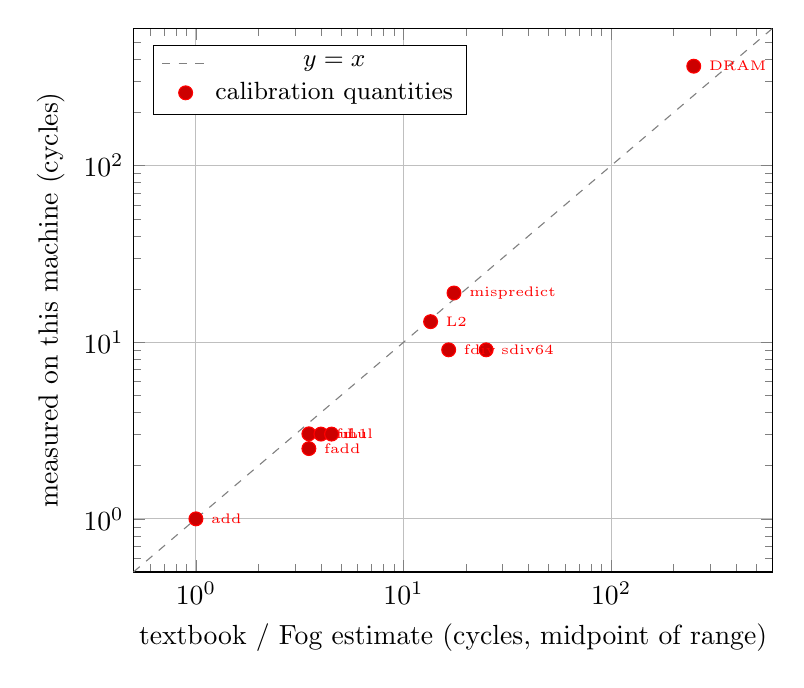
\begin{tikzpicture}
\begin{axis}[width=0.8\textwidth, height=0.7\textwidth, xmode=log, ymode=log, xlabel={textbook / Fog estimate (cycles, midpoint of range)}, ylabel={measured on this machine (cycles)}, grid=major,
  xmin=0.5, xmax=600, ymin=0.5, ymax=600, legend pos=north west, legend style={font=\small}]
\addplot[gray, dashed, domain=0.5:600] {x};
\addlegendentry{$y = x$}
\addplot+[only marks, mark=*, mark size=2.5pt, nodes near coords, point meta=explicit symbolic, nodes near coords style={font=\tiny, anchor=west, xshift=2pt}] coordinates {(1.0,1.00) [add] (3.5,3.03) [mul] (25.0,9.06) [sdiv64] (3.5,2.50) [fadd] (4.0,3.02) [fmul] (16.5,9.06) [fdiv] (4.5,3.02) [L1] (13.5,13.08) [L2] (250.0,365.79) [DRAM] (17.5,19.01) [mispredict]};
\addlegendentry{calibration quantities}
\end{axis}
\end{tikzpicture}